%%%%%%%%%%%%%%%%%%%%%%%%%%%%%%%%%%%%%%%%%%%%%%%%%%%%%%%%%%%%%%%%%%%%
% This is a thesis template for Gebze Technical University.
%
% Please only edit the areas proceeded by a comment starting with %%
% otherwise the template may be broken.
%
% This file is only to be used for editing the general fields
% and inputting the body of the thesis in the designated areas.
% Please write the body of the thesis in separate files, and input
% them as shown in the comment preceding the area.
%
% Created in Aug 2021 by Usama Derbashi.
%%%%%%%%%%%%%%%%%%%%%%%%%%%%%%%%%%%%%%%%%%%%%%%%%%%%%%%%%%%%%%%%%%%%
\documentclass[12pt]{report}


% Language and typeset setting
\usepackage[english]{babel}
\usepackage[a4paper,top=25mm,bottom=25mm,left=40mm,right=25mm]{geometry}
\usepackage[onehalfspacing]{setspace}
\usepackage{algorithm, algpseudocode}
\usepackage{indentfirst}
\setlength{\parindent}{1cm}
\setlength{\abovecaptionskip}{12pt plus 0pt minus 0pt}
\setlength{\belowcaptionskip}{12pt plus 0pt minus 0pt}
\setlength{\textfloatsep}{18.0pt plus 0.0pt minus 0.0pt}
\setlength{\floatsep}{18.0pt plus 0.0pt minus 0.0pt}
\setlength{\intextsep}{18.0pt plus 0.0pt minus 0.0pt}
\setlength{\skip\footins}{18.0pt plus 0.0pt minus 0.0pt}

% Core packages and settings
\usepackage[colorlinks=false]{hyperref}
\usepackage{amsmath}

\usepackage{titlesec} %setting the titles of chapters and sections
\setcounter{secnumdepth}{4}
\setcounter{tocdepth}{4}
\titleformat{\chapter}[hang]{\normalfont\bfseries\MakeUppercase}{}{0pt}{\LARGE\thechapter. }
\titleformat{\section}[hang]{\normalfont\bfseries}{}{0pt}{\Large\thesection. }
\titleformat{\subsection}[hang]{\normalfont\bfseries}{}{0pt}{\large\thesubsection. }
\titleformat{\subsubsection}[hang]{\normalfont\bfseries}{}{0pt}{\large\thesubsubsection. }
\titlespacing*{\chapter}{0pt}{0pt}{18pt}
\titlespacing*{\section}{0pt}{18pt}{18pt}
\titlespacing*{\subsection}{0pt}{18pt}{18pt}
\titlespacing*{\subsubsection}{0pt}{18pt}{18pt}

\usepackage{graphicx}
\graphicspath{{./Imgs/}} %pointing the directory of images

\usepackage{fancyhdr} % setting footers
\usepackage{etoolbox} 
\renewcommand{\headrulewidth}{0pt}
\patchcmd{\chapter}{\thispagestyle{plain}}{\thispagestyle{fancy}}{}{}
\pagestyle{fancy}
\fancyhf{}
\fancyfoot[C]{\fontsize{11pt}{11pt}\thepage}

\usepackage[style=ieee]{biblatex}
\addbibresource{refs.bib}
\usepackage{csquotes}% Needed for babel(in biblatex)

\usepackage[bottom, perpage]{footmisc}%% amkes footnotes at the bottom

\usepackage{GTUThesis}


% Additional packages if needed
%% For the sake of not messing the template add them here
\usepackage{lipsum}


% Important information
%% Make sure to enter all the info below
\title{Project Title}
\author{Student Name}
\faculty{Faculty of Engineering}
\department{Computer Engineering Department}
\supervisor{Prof. XXXXX YYYYY}
\theyear{2022}


\begin{document}

%Front Matter
\pagenumbering{roman} %start with roman numbering 
\projecttitlepageenglish
\maketitle
\setcounter{page}{3} %the first two title pages are not counted so this is a buffer
\begin{outertitles} % makes titles centred

%% below enter as follows 
%% {DATE_OF_DEMO}{JURY}
%% Note that JURY should be comma separated
\makejury{31/08/2021}{Prof. Erchan Aptoula, M.Sc Melike Ilteralp}
\chapter*{Abstract}
\addcontentsline{toc}{chapter}{Abstract}

%% Edit below this line
Lorem Ipsum is simply dummy text of the printing and typesetting industry. Lorem Ipsum has been the industry's standard dummy text ever since the 1500s, when an unknown printer took a galley of type and scrambled it to make a type specimen book. It has survived not only five centuries, but also the leap into electronic typesetting, remaining essentially unchanged. It was popularised in the 1960s with the release of Letraset sheets containing Lorem Ipsum passages, and more recently with desktop publishing software like Aldus PageMaker including versions of Lorem Ipsum.

%% Until here
\vfill
%% Edit after {Keywords:}
\textbf{Keywords:} keyword1, keyword2.
\clearpage
\chapter*{Özet}
\addcontentsline{toc}{chapter}{Özet}

%% Edit below this line
Lorem Ipsum is simply dummy text of the printing and typesetting industry. Lorem Ipsum has been the industry's standard dummy text ever since the 1500s, when an unknown printer took a galley of type and scrambled it to make a type specimen book. It has survived not only five centuries, but also the leap into electronic typesetting, remaining essentially unchanged. It was popularised in the 1960s with the release of Letraset sheets containing Lorem Ipsum passages, and more recently with desktop publishing software like Aldus PageMaker including versions of Lorem Ipsum.

%% Until here
\vfill
%% Edit after {Anahtar Kelimeler:}
\textbf{Anahtar Kelimeler:} anahtar kelime1, anahtar kelime2.
\clearpage
\chapter*{Acknowledgement}
\addcontentsline{toc}{chapter}{Acknowledgement}

%% Edit below this line
Thank you mate!!



%% Until here
\vspace{1cm}
\begin{flushright}
\textbf{Name Surname} %% your name here
\end{flushright}
\clearpage
\chapter*{List of Symbols and Abbreviations}
\addcontentsline{toc}{chapter}{List of Symbols and Abbreviations}

\begin{tabular}{lcl}
    \textbf{Symbol or}&&\\
    \textbf{Abbreviation} &:& \textbf{Explanation}\\
    
    %% Edit below in the format
    %% XYZ &:& EXPLANATION\\
    %% where XYZ is the acronym or symbol
    %% and EXPLANATION is the explanation of it
    %% make sure not to forget &:& between them, and \\ at the end of EXPLANATION
    
    ABC &:& The first three letters in the English alphabet\\
    $\mu$ &:& Small mu\\
    
    %% Until here
\end{tabular}

\clearpage

\tableofcontents
\addcontentsline{toc}{chapter}{Contents}
\clearpage

\listoffigures
\addcontentsline{toc}{chapter}{List of Figures}
\clearpage

\listoftables
\addcontentsline{toc}{chapter}{List of Tables}
\clearpage

\end{outertitles}
\fancyhf{}%reset footer
\fancyfoot[R]{\fontsize{11pt}{11pt}\thepage}%page numbers in the corner
\addtocontents{toc}{\protect\vspace{18pt}}
\pagenumbering{arabic}%turn to arabic numbers

% Mainmatter

%% Only input files, don't write here
%% \input{./Body/Mainmatter/FILE}
\chapter{A Chapter}

Lorem Ipsum is simply dummy text of the printing and typesetting industry. Lorem Ipsum has been the industry's standard dummy text ever since the 1500s, when an unknown printer took a galley of type and scrambled it to make a type specimen book. It has survived not only five centuries, but also the leap into electronic typesetting, remaining essentially unchanged. It was popularised in the 1960s with the release of Letraset sheets containing Lorem Ipsum passages, and more recently with desktop publishing software like Aldus PageMaker including versions of Lorem Ipsum. \ref{fig:frog}.

\begin{figure}[!htbp]
    \centering
    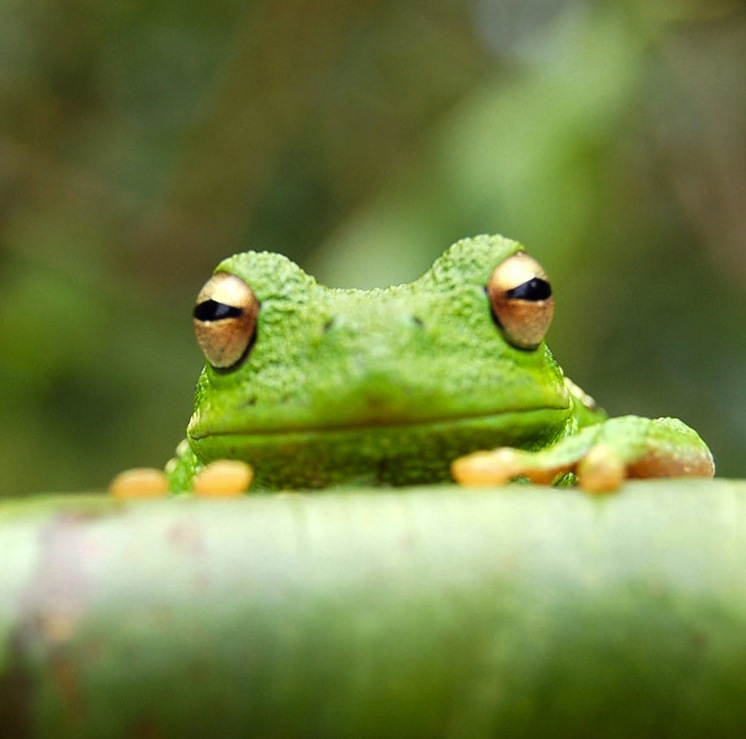
\includegraphics[width=0.3\textwidth]{frog.jpg}
    \caption{\label{fig:frog}This frog was uploaded via the file-tree menu.}
\end{figure}

\section{A Section}

It is a long established fact that a reader will be distracted by the readable content of a page when looking at its layout. The point of using Lorem Ipsum is that it has a more-or-less normal distribution of letters, as opposed to using 'Content here, content here', making it look like readable English. Many desktop publishing packages and web page editors now use Lorem Ipsum as their default model text, and a search for 'lorem ipsum' will uncover many web sites still in their infancy. Various versions have evolved over the years, sometimes by accident, sometimes on purpose (injected humour and the like). \footnote{footnotes working fine}\footnote{footnotes are working fine?}\footnote{lets hope footnotes working fine}

\section{B Section}

\subsection{A Subsection}
There are many variations of passages of Lorem Ipsum available, but the majority have suffered alteration in some form, by injected humour, or randomised words which don't look even slightly believable. If you are going to use a passage of Lorem Ipsum, you need to be sure there isn't anything embarrassing hidden in the middle of text. 

\subsubsection{A Subsubsection}
The generated Lorem Ipsum is therefore always free from repetition, injected humour, or non-characteristic words etc.

\subsection{B subsection}
The standard chunk of Lorem Ipsum used since the 1500s is reproduced below for those interested. Sections 1.10.32 and 1.10.33 from "de Finibus Bonorum et Malorum" by Cicero are also reproduced in their exact original form, accompanied by English versions from the 1914 translation by H. Rackham.\footnote{footnotes working fine}\footnote{footnotes are working fine?}\footnote{lets hope footnotes working fine}

\section{C Section}
Lorem ipsum dolor sit amet, consectetur adipiscing elit, sed do eiusmod tempor incididunt ut labore et dolore magna aliqua. Ut enim ad minim veniam, quis nostrud exercitation ullamco laboris nisi ut aliquip ex ea commodo consequat. Duis aute irure dolor in reprehenderit in voluptate velit esse cillum dolore eu fugiat nulla pariatur. Excepteur sint occaecat cupidatat non proident, sunt in culpa qui officia deserunt mollit anim id est laborum. \ref{tab:widgets} \cite{One, Two, Three}.

\begin{table}[!htbp]
    \centering
    \caption{\label{tab:widgets}An example table.}
    \begin{tabular}{l|r}
        Item & Quantity \\\hline
        Widgets & 45 \\
        Gadgets & 13
    \end{tabular}
\end{table}
\chapter{B Chapter}

On the other hand, we denounce with righteous indignation and dislike men who are so beguiled and demoralized by the charms of pleasure of the moment, so blinded by desire, that they cannot foresee the pain and trouble that are bound to ensue; and equal blame belongs to those who fail in their duty through weakness of will, which is the same as saying through shrinking from toil and pain. These cases are perfectly simple and easy to distinguish. \ref{fig:frogger}\ref{fig:froggerr}.

\begin{figure}[!htbp]
    \centering
    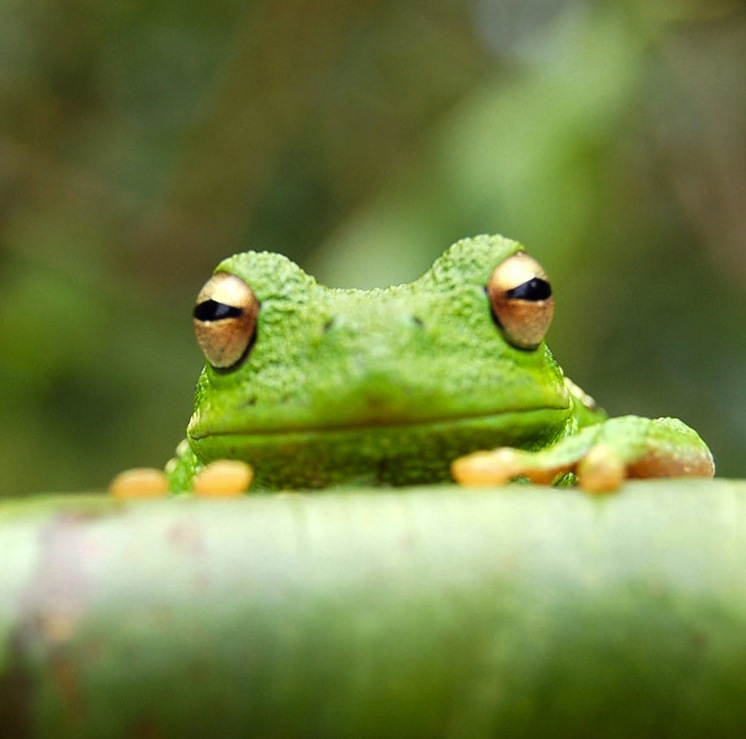
\includegraphics[width=0.3\textwidth]{frog.jpg}
    \caption{\label{fig:frogger}Another instance of the frog.}
\end{figure}
\begin{figure}[!htbp]
    \centering
    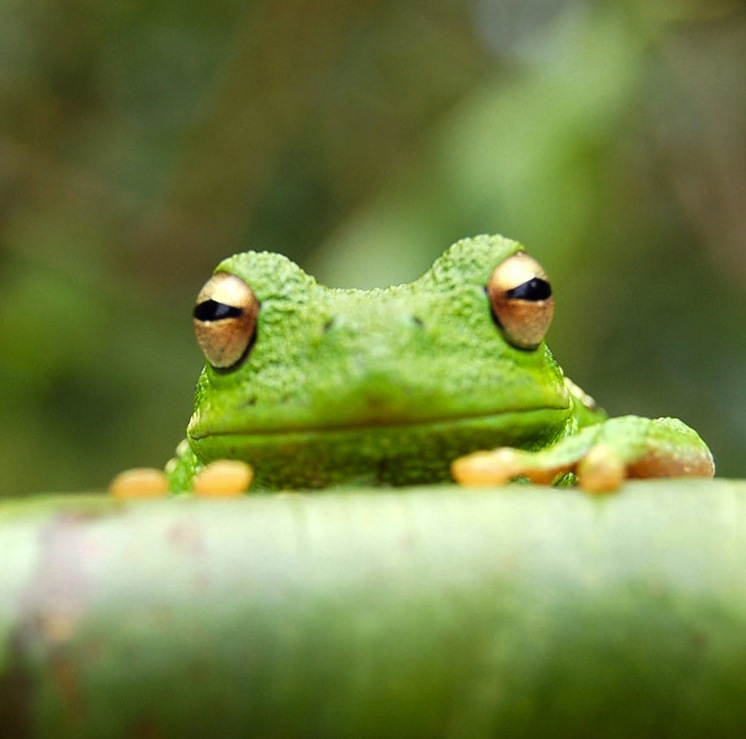
\includegraphics[width=0.3\textwidth]{frog.jpg}
    \caption{\label{fig:froggerr}And a third one.}
\end{figure}

\section{A Section}

In a free hour, when our power of choice is untrammelled and when nothing prevents our being able to do what we like best, every pleasure is to be welcomed and every pain avoided. But in certain circumstances and owing to the claims of duty or the obligations of business it will frequently occur that pleasures have to be repudiated and annoyances accepted. The wise man therefore always holds in these matters to this principle of selection: he rejects pleasures to secure other greater pleasures, or else he endures pains to avoid worse pains.

\section{B Section}

\subsection{A Subsection}
The Algorithm \ref{labelOfAlgorithm} shows the pseudo code of...

\begin{algorithm}
\caption{Caption of the algorithm}
\label{labelOfAlgorithm}
\begin{algorithmic}
\Require $n \geq 0$ % i.e. input
\Ensure $y = x^n$  % i.e. output
\State $y \gets 1$
\State $X \gets x$
\State $N \gets n$
\While{$N \neq 0$}
\If{$N$ is even}
    \State $X \gets X \times X$
    \State $N \gets \frac{N}{2}$  \Comment{This is a comment}
\ElsIf{$N$ is odd}
    \State $y \gets y \times X$
    \State $N \gets N - 1$
\EndIf
\EndWhile
\end{algorithmic}
\end{algorithm}


\subsubsection{A Subsubsection}
Excepteur sint occaecat cupidatat non proident, sunt in culpa qui officia deserunt mollit anim id est laborum.
\subsection{B subsection}
Sed ut perspiciatis unde omnis iste natus error sit voluptatem accusantium doloremque laudantium, totam rem aperiam, eaque ipsa quae ab illo inventore veritatis et quasi architecto beatae vitae dicta sunt explicabo. Nemo enim ipsam voluptatem quia voluptas sit aspernatur aut odit aut fugit, sed quia consequuntur magni dolores eos qui ratione voluptatem sequi nesciunt. Neque porro quisquam est, qui dolorem ipsum quia dolor sit amet, consectetur, adipisci velit, sed quia non numquam eius modi tempora incidunt ut labore et dolore magnam aliquam quaerat voluptatem. 

\section{C Section}
Ut enim ad minima veniam, quis nostrum exercitationem ullam corporis suscipit laboriosam, nisi ut aliquid ex ea commodi consequatur? Quis autem vel eum iure reprehenderit qui in ea voluptate velit esse quam nihil molestiae consequatur, vel illum qui dolorem eum fugiat quo voluptas nulla pariatur? \ref{tab:widgetss} \cite{One, Two, Three}.

\begin{table}[!htbp]
\centering
\caption{\label{tab:widgetss}Comparison of percentages.}
\begin{tabular}{c|cc|cc}
\hline
Mode &  \multicolumn{2}{c}{Var} & \multicolumn{2}{c}{Cum}\\ 
\hline
1   &  17.5 & 19.1   & 17.5  & 19.1\\
2   &  11.8 & 12.7   & 29.3  & 31.9\\
3   &  6.6  &  5.6   & 35.9  & 37.4\\
\end{tabular}
\end{table}

\begin{enumerate}
\item first,
\item second.
\end{enumerate}
\dots and bullet points \dots
\begin{itemize}
\item one bullet,
\item two bullets.
\end{itemize}

Let $X_1, X_2, \ldots, X_n$ be a sequence of independent and identically distributed random variables with $\text{E}[X_i] = \mu$ and $\text{Var}[X_i] = \sigma^2 < \infty$, and let
\[S_n = \frac{X_1 + X_2 + \cdots + X_n}{n}
      = \frac{1}{n}\sum_{i}^{n} X_i\]
denote their mean. Then as $n$ approaches infinity, the random variables $\sqrt{n}(S_n - \mu)$ converge in distribution to a normal $\mathcal{N}(0, \sigma^2)$.

\begin{quote}
    At vero eos et accusamus et iusto odio dignissimos ducimus qui blanditiis praesentium voluptatum deleniti atque corrupti quos dolores et quas molestias excepturi sint occaecati cupiditate non provident, similique sunt in culpa qui officia deserunt mollitia animi, id est laborum et dolorum fuga.
\end{quote}
\chapter{Conclusions}
Lorem ipsum dolor sit amet, consectetur adipiscing elit, sed do eiusmod tempor incididunt ut labore et dolore magna aliqua. Ut enim ad minim veniam, quis nostrud exercitation ullamco laboris nisi ut aliquip ex ea commodo consequat. Duis aute irure dolor in reprehenderit in voluptate velit esse cillum dolore eu fugiat nulla pariatur. 




% DON'T INPUT FILES AFTER HERE
\begin{outertitles}
\clearpage
\setlength{\emergencystretch}{1em}
\printbibliography
\addtocontents{toc}{\protect\vspace{18pt}}
\addcontentsline{toc}{chapter}{Bibliography}
%% If you don't want a CV or appendices add a % at the beginning of the relevant line
\chapter*{CV}
\addcontentsline{toc}{chapter}{CV}

%% Edit below this line
XXX.



%% Until here
\clearpage
\chapter*{Appendices}
\addcontentsline{toc}{chapter}{Appendices}

\section*{Appendix 1: Some publications}

No one significant, in AAA.

\section*{Appendix 2: Some explanation}

None needed mate!
\end{outertitles}
\end{document}